\subsection{Modulo de comunicación}

	Si consideramos la lista de elementos dinámicos y cada estado que pueden admitir, es claro que la cantidad de señales sobrepasaría por mucho la limitada cantidad de puertos que una FPGA pueda proveer. Es por eso que se decidió que la información deberá ser recibida por la FPGA y transmitida desde la FPGA en formato serie. El formato serie es ampliamente utilizado en las redes ferroviarias, por ejemplo RS-485 o MVB en las redes de comunicación de trenes  TCN [REF]. Esta comunicación deberá ser flexible para ser utilizada en diferentes implementaciones con menor o mayor demanda de recursos.
	
	En la Figura \ref{fig:GeneralCom} se presenta la propuesta de conexión de la FPGA con una computadora externa, junto con los módulos internos de comunicación.	La UART (del inglés \textit{Universal Asynchronous Receiver-Transmitter}) es la unidad encargada de recibir y transmitir las tramas de datos entre la FPGA y la computadora.
	
	\begin{figure}[H]
		\centering
		\includegraphics[width=1\textwidth]{example-image}
		\centering\caption{FPGA.}
		\label{fig:GeneralCom}
	\end{figure}
	
	El bloque de recepción UART es el encargado de procesar las tramas con un baudrate preestablecido y almacenar el valor de la trama en la FIFO de entrada. La trama será enviada al sistema de enclavamientos, junto con una serie de pulsos para indicar cuándo deben ser leídos. El sistema de enclavamientos la procesará y devolverá una nueva trama a la FIFO de salida. Finalmente la nueva trama será enviada a la UART de tramisión que enviará la información con el mismo baudrate que fue recibido.
		
	En la Figura \ref{fig:Stream} se ilustra el formato definido para las tramas de entrada y salida. La trama tendrá un tamaño de entrada N y de salida M, con N menor que M, debido a que el estado de ocupación de las vías es de sólo lectura. Además, la trama tendrá un caracter delimitador de entrada y de salida ($<$ y $>$ respectivamente). Todos los elementos de la trama serán en formato ASCII, para poder ser interpretados fácilmente en una terminal y ser menos susceptibles a errores por alteraciones en algún bit aleatorio.
	
	\begin{figure}[H]
		\centering
		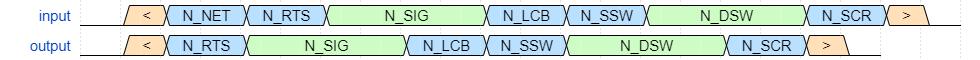
\includegraphics[width=1\textwidth]{Figuras/Tramas.png}
		\centering\caption{Tramas de entrada y salida.}
		\label{fig:Stream}
	\end{figure}
	
	De la lista de estados de cada elemento dinámico dado anteriormente se deduce que cada elemento requiere un sólo caractér para definir su estado, salvo los semáforos y cambios de vías dobles, que necesitan dos caracteres. Por lo tanto, el largo de la trama de entrada y de salida queda definido por la Fórmula \ref{eq:StreamLength_in} y la Fórmula \ref{eq:StreamLength_out}, respectivamente.
	
	\begin{equation} 
		\label{eq:StreamLength_in}
		\text{N} = 1\text{bit} (\text{N}_{NET}+\text{N}_{\text{RTS}}+\text{N}_{\text{LCB}}+\text{N}_{\text{SSW}}+\text{N}_{\text{SCR}})+2\text{bits} (\text{N}_{\text{SIG}}+\text{N}_{\text{DSW}})
	\end{equation}
	
	\begin{equation} 
		\label{eq:StreamLength_out}
		\text{M} = 1\text{bit} (\text{N}_{\text{RTS}}+\text{N}_{\text{LCB}}+\text{N}_{\text{SSW}}+\text{N}_{\text{SCR}})+2\text{bits} (\text{N}_{\text{SIG}}+\text{N}_{\text{DSW}})
	\end{equation}
	
	La implementación de los módulos de transmisión y recepción de la UART es invariante para cada locación, es decir, los recursos asignados serán los mismos, cualquiera sea el tamaño del sistema a implementar. Los módulos de memorias FIFO, en cambio, dependen de las características y del tamaño del sistema. Locaciones mas complejas tendrán valores de N y M mayores y, por lo tanto, requerirán FIFOs mas grandes. 
	
	Con este criterio de diseño, en todos los demás casos, la FIFO de salida tendrá el mismo tamaño que la FIFO de entrada o a lo sumo será 50 \% menor, lo que representa un ahorro de 25 \% de los recursos estimados. Por ejemplo, si se necesita que la entrada tenga 15 bits y la salida 7 bits y se le asignara el mismo tamaño a ambas FIFOs; tanto la FIFO de entrada como la de salida necesitarán 16 bits cada una, dando un total de 32 bits. Pero si se aplica el criterio de tamaños desacoplados, entonces para la FIFO de salida podrían asignarse solamente 8 bits,
	dando un total de 24 bits, un 25 \% menos que los 32 bits que necesitaría si ambas FIFOs quedaran definidas según los datos de la entrada.
	
\subsection{Módulo Detector}
	\label{sec:detector}
	
	El módulo \textit{detector} es el encargado de detectar el inicio y final de cada trama, validando que el contenido de la misma tenga N caracteres, conforme al formato de trama expuesto en la Sección \ref{sec:UART}. A medida que la validación tiene lugar, los caracteres ASCII son convertidos en valores booleanos (\textit{std\_logic}) dentro de un vector de elementos booleanos llamado \textit{packet}[N] (\textit{std\_logic\_vector} de N elementos). El diagrama de bloques de las máquinas de estado finitas con camino de datos se muestra en la Figura \ref{fig:Detector_module}.
	
	\begin{figure}[H]
		\centering
		\includegraphics[width=1\textwidth]{Figuras/Detector_module.png}
		\centering\caption{FSMD del módulo \textit{Detector}.}
		\label{fig:Detector_module}
	\end{figure}
	
	En cada pulso de reloj (\textit{clk\_i}), el módulo UART envía un caracter por medio de la señal \textit{r\_data} (8 bytes) y un pulso (\textit{r\_available}) para informar que un nuevo dato ha sido enviado. El pulso de reloj es utilizado principalmente en el módulo \textit{Counter\_0\_to\_N}, cuyo parámetro N ya ha sido calculado por el ACG previo a generar el código y es la cantidad de caracteres que serán enviados a continuación del caracter de inicio. El proceso de detección y validación de la trama recibida se describe el diagrama de estados de la Figura \ref{fig:Detector_FSMD}.
	
	\begin{figure}[H]
		\centering
		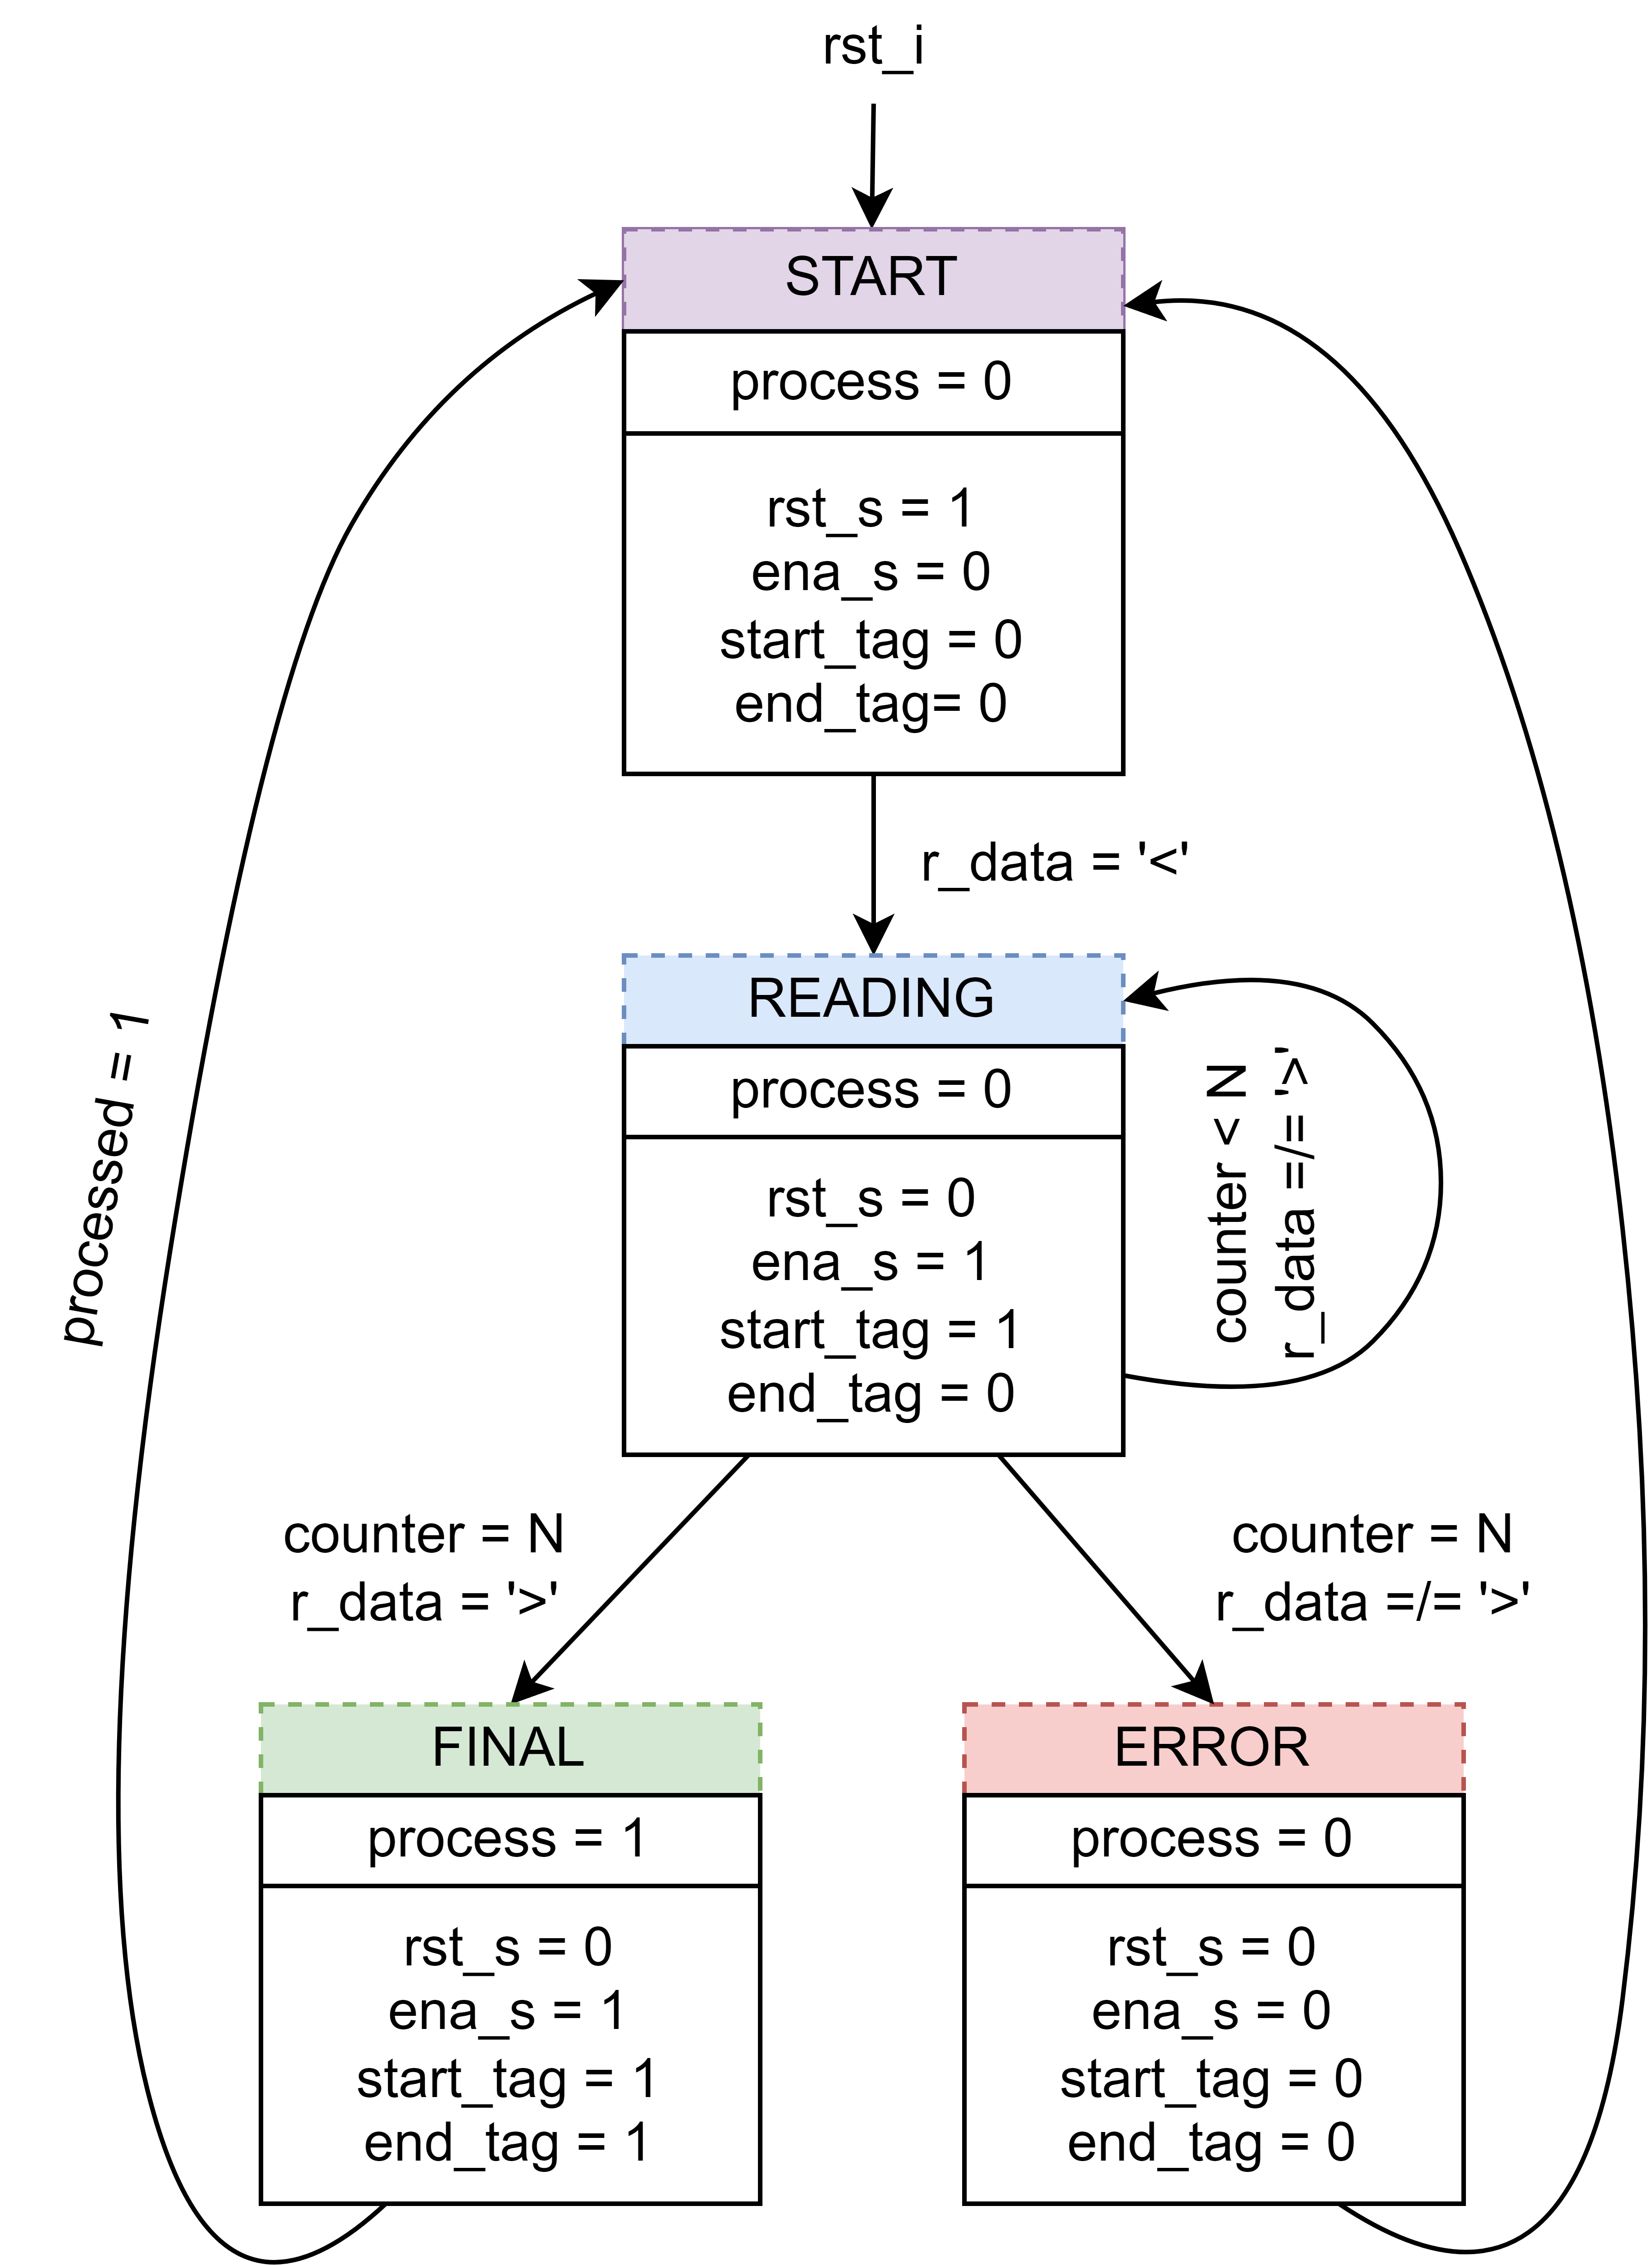
\includegraphics[width=0.8\textwidth]{Figuras/Detector_FSMD.png}
		\centering\caption{Diagrama de estados del módulo \textit{Detector}.}
		\label{fig:Detector_FSMD}
	\end{figure}
	
	El módulo \textit{Detector} inicia por detecto en el estado \textit{start}, aguardando por el caracter de inicio de trama '$<$'. Al recibir el caracter de inicio de trama, el módulo transiciona al estado \textit{reading}. En el estado \textit{reading} se recibirán solamente los caracteres ASCII '0' y '1'. Si al terminar de recibir N caracteres, el próximo caracter no es el de fin de trama '$>$' entonces se transiciona al estado \textit{error}, se reinician las variables auxiliares, la trama se descarta y se vuelve al estado \textit{start}.
	
	Si el próximo caracter luego de leer N valores ASCII '0' y '1' es el caracter de fin de trama '$>$', entonces el módulo transiciona al estado \textit{final}, donde se da por válida la trama y se habilita su envío al módulo \textit{decoder}, para volver al estado \textit{start} a la espera de un nuevl caracter de inicio de trama, reiniciando todas las variables auxiliares.
	
	Internamente se tienen diversas variables auxiliares para controlar si se han recibido los delimitadores y si la cantidad recibida es correcta. Eso cobra gran importancia al realizar los ensayos, porque se puede diferenciar rápidamente la fuente de posibles errores.
\subsection{Módulo Decoder}
	\label{sec:decoder}
	
	El módulo \textit{Decoder} (ver Figura \ref{fig:GeneralSystem}) es el encargado de demultiplexar la trama \textit{packet}[N] ya validada por el módulo \textit{Detector}. El módulo \textit{Decoder} recibe el vector de elementos booleanos \textit{packet}[N] y la señal \textit{process} que indica cuando puede iniciar el proceso de demultiplexación. La salida serán todos los vectores de estado de los elementos ferroviarios. El diagrama de bloques de la máquinas de estado finitas con camino de datos se muestra en la Figura \ref{fig:Decoder_module}. En este caso particular, no se cuenta con una máquina de estados, ya que la demultiplexación se realiza directamente.
	
	\begin{figure}[H]
		\centering
		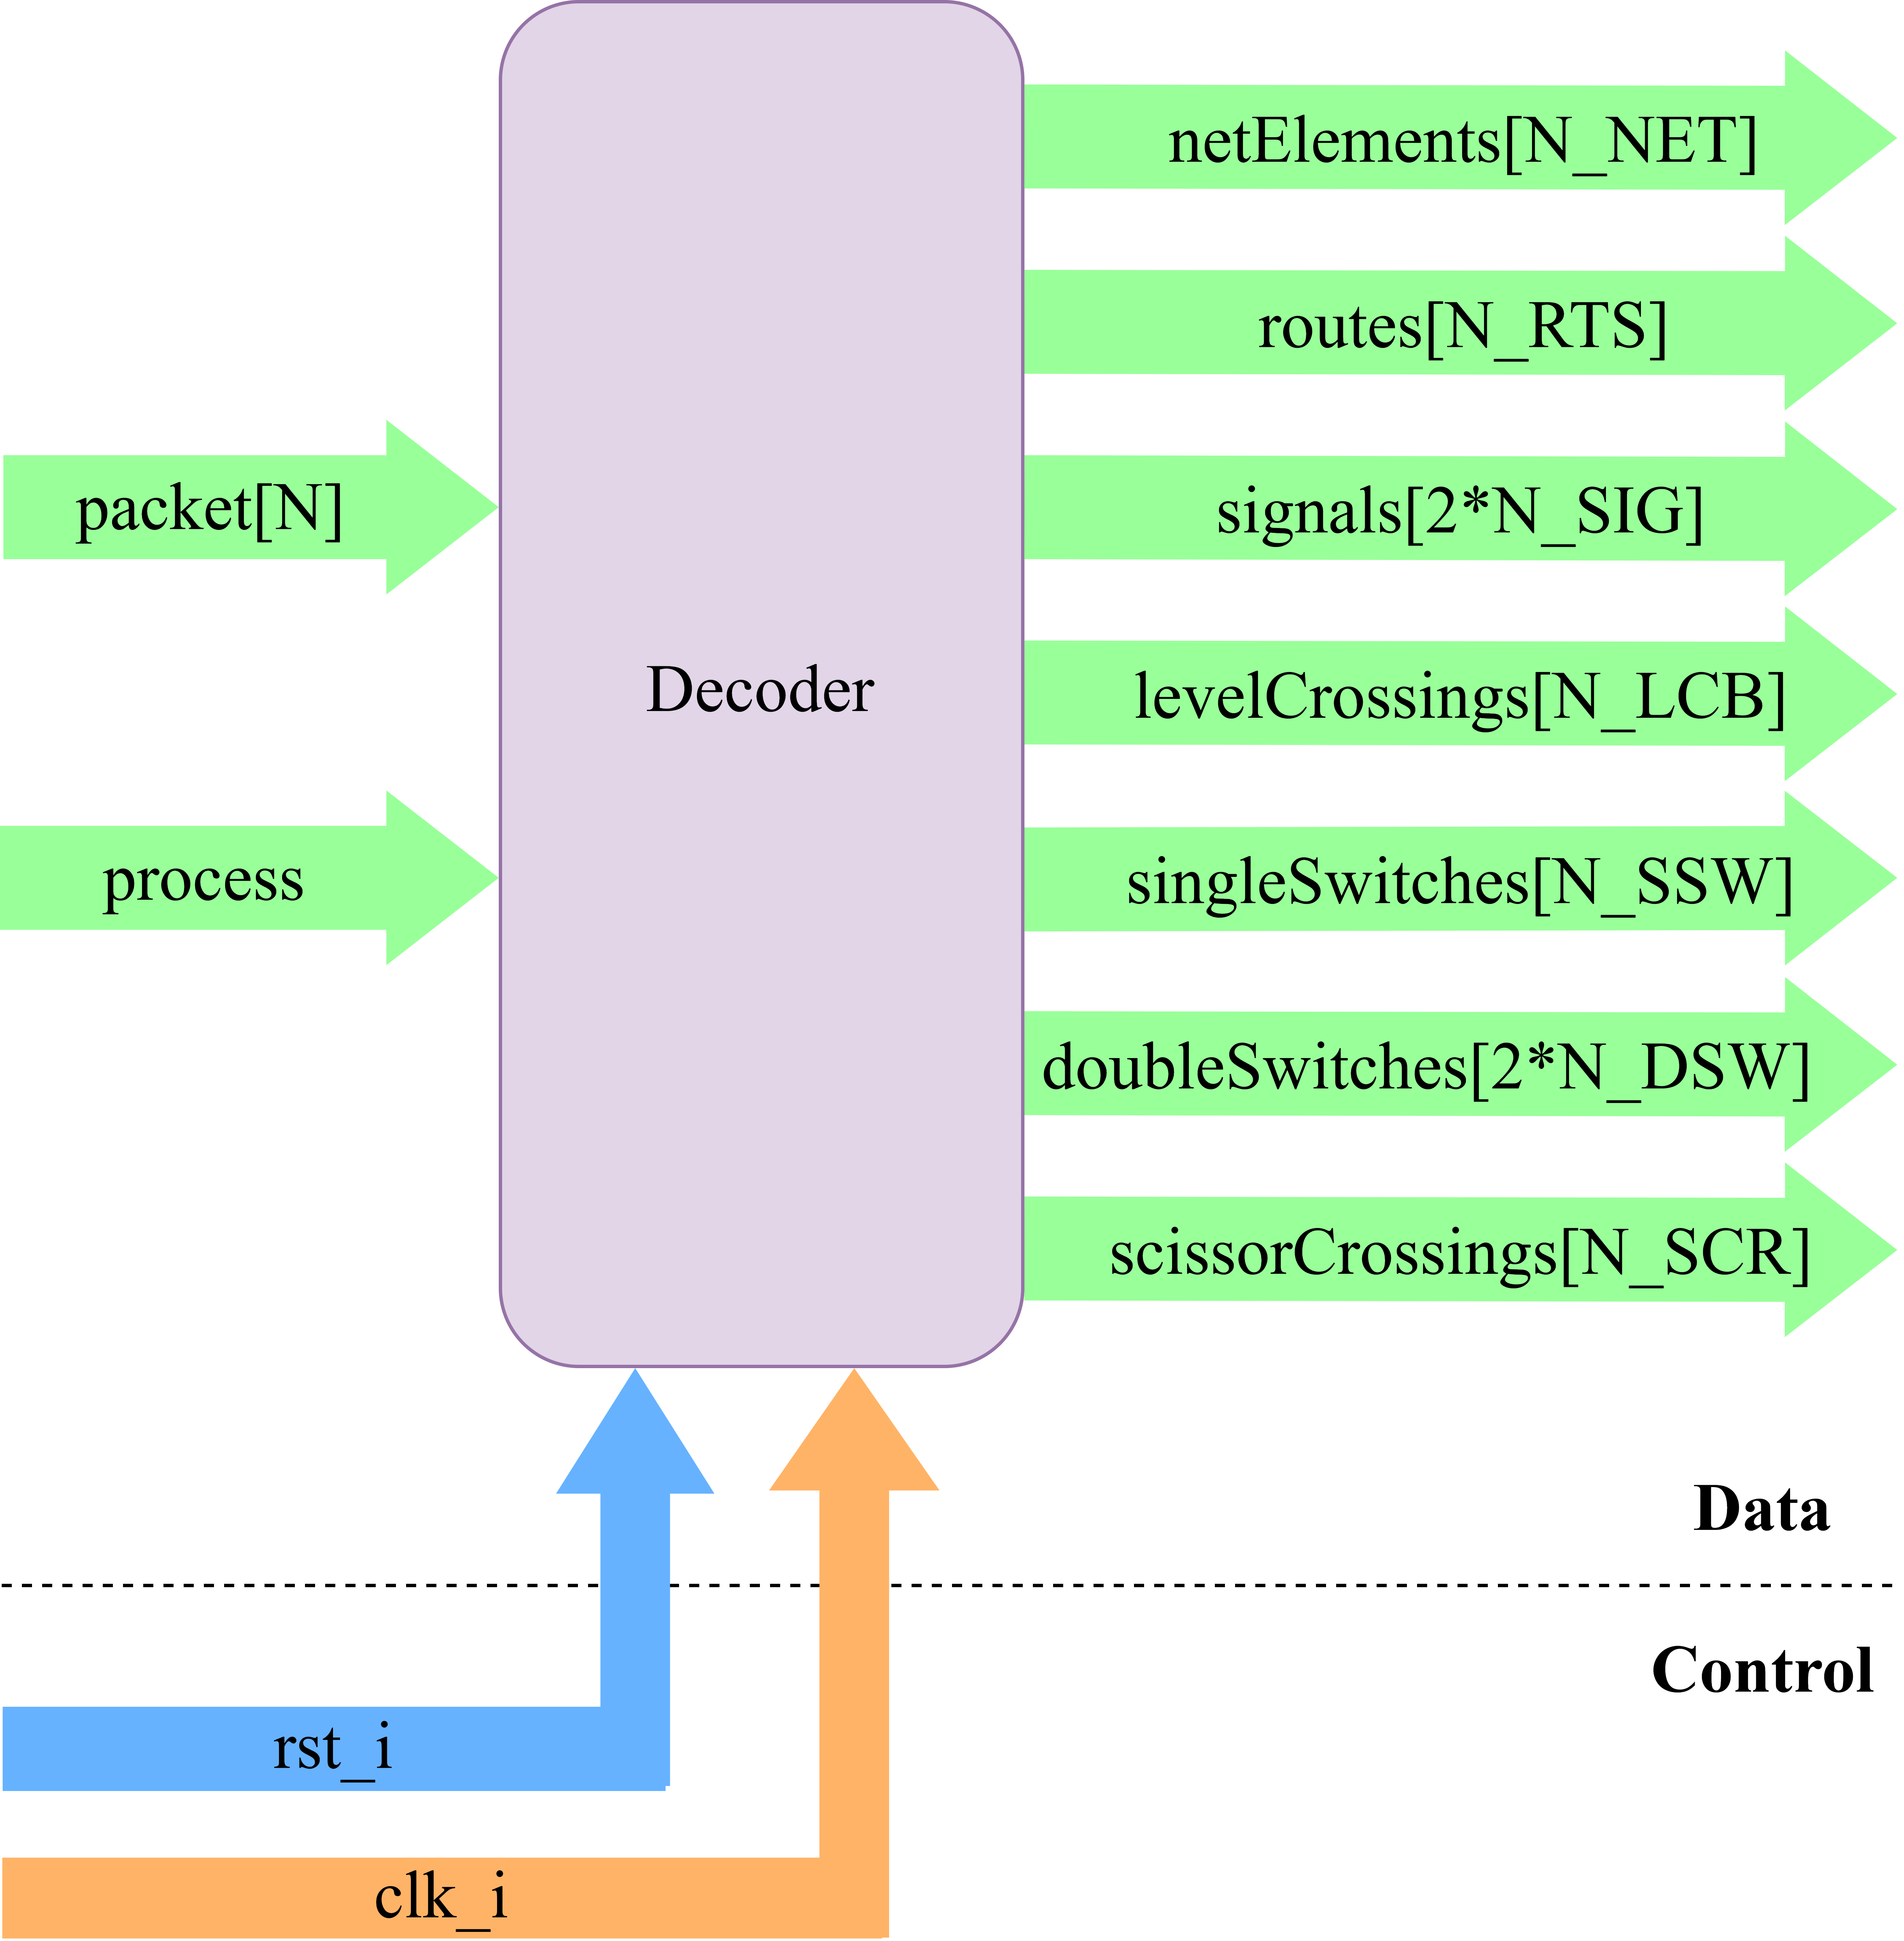
\includegraphics[width=1\textwidth]{Figuras/Decoder_module.png}
		\centering\caption{FSMD del módulo \textit{Decoder}.}
		\label{fig:Decoder_module}
	\end{figure}
	
	 La porción de \textit{packet}[N] correspondiente a cada vector será en función de la cantidad de elementos de cada tipo presentes en la locación. Esto ya fue calculado previamente por el ACG y explicado en la Sección \ref{sec:UART} al definir el formato de la trama. Si la cantidad de un cierto elemento ferroviario es mayor que uno, el ACG implementará el estado de ese elemento con un vector hexadecimal del tamaño adecuado. Si solo existe un elemento ferroviario de ese tipo, el ACG implementará un escalar hexadecimal. Si no existiese ningún elemento ferroviario en la locación, el ACG no implementará ninguna de las funcionalidades relativas a dicho elemento, optimizando el uso de recursos en la FPGA.
\subsection{Módulo Encoder}
	\label{sec:encoder}
	
	El módulo \textit{Encoder} (ver Figura \ref{fig:GeneralSystem}) es el encargado de multiplexar los vectores de estado provenientes del módulo \textit{Network} y reconstruir una nueva trama, esta vez sin los valores de ocupación de vías por ser de sólo lectura. Esta nueva trama será \textit{packet}[N], junto con la señal \textit{processed} para indicar al módulo \textit{Printer} que la trama está completa y lista para ser transmitida. El diagrama de bloques de las máquinas de estado finitas con camino de datos se muestra en la Figura \ref{fig:Encoder_module}.
	
	\begin{figure}[H]
		\centering
		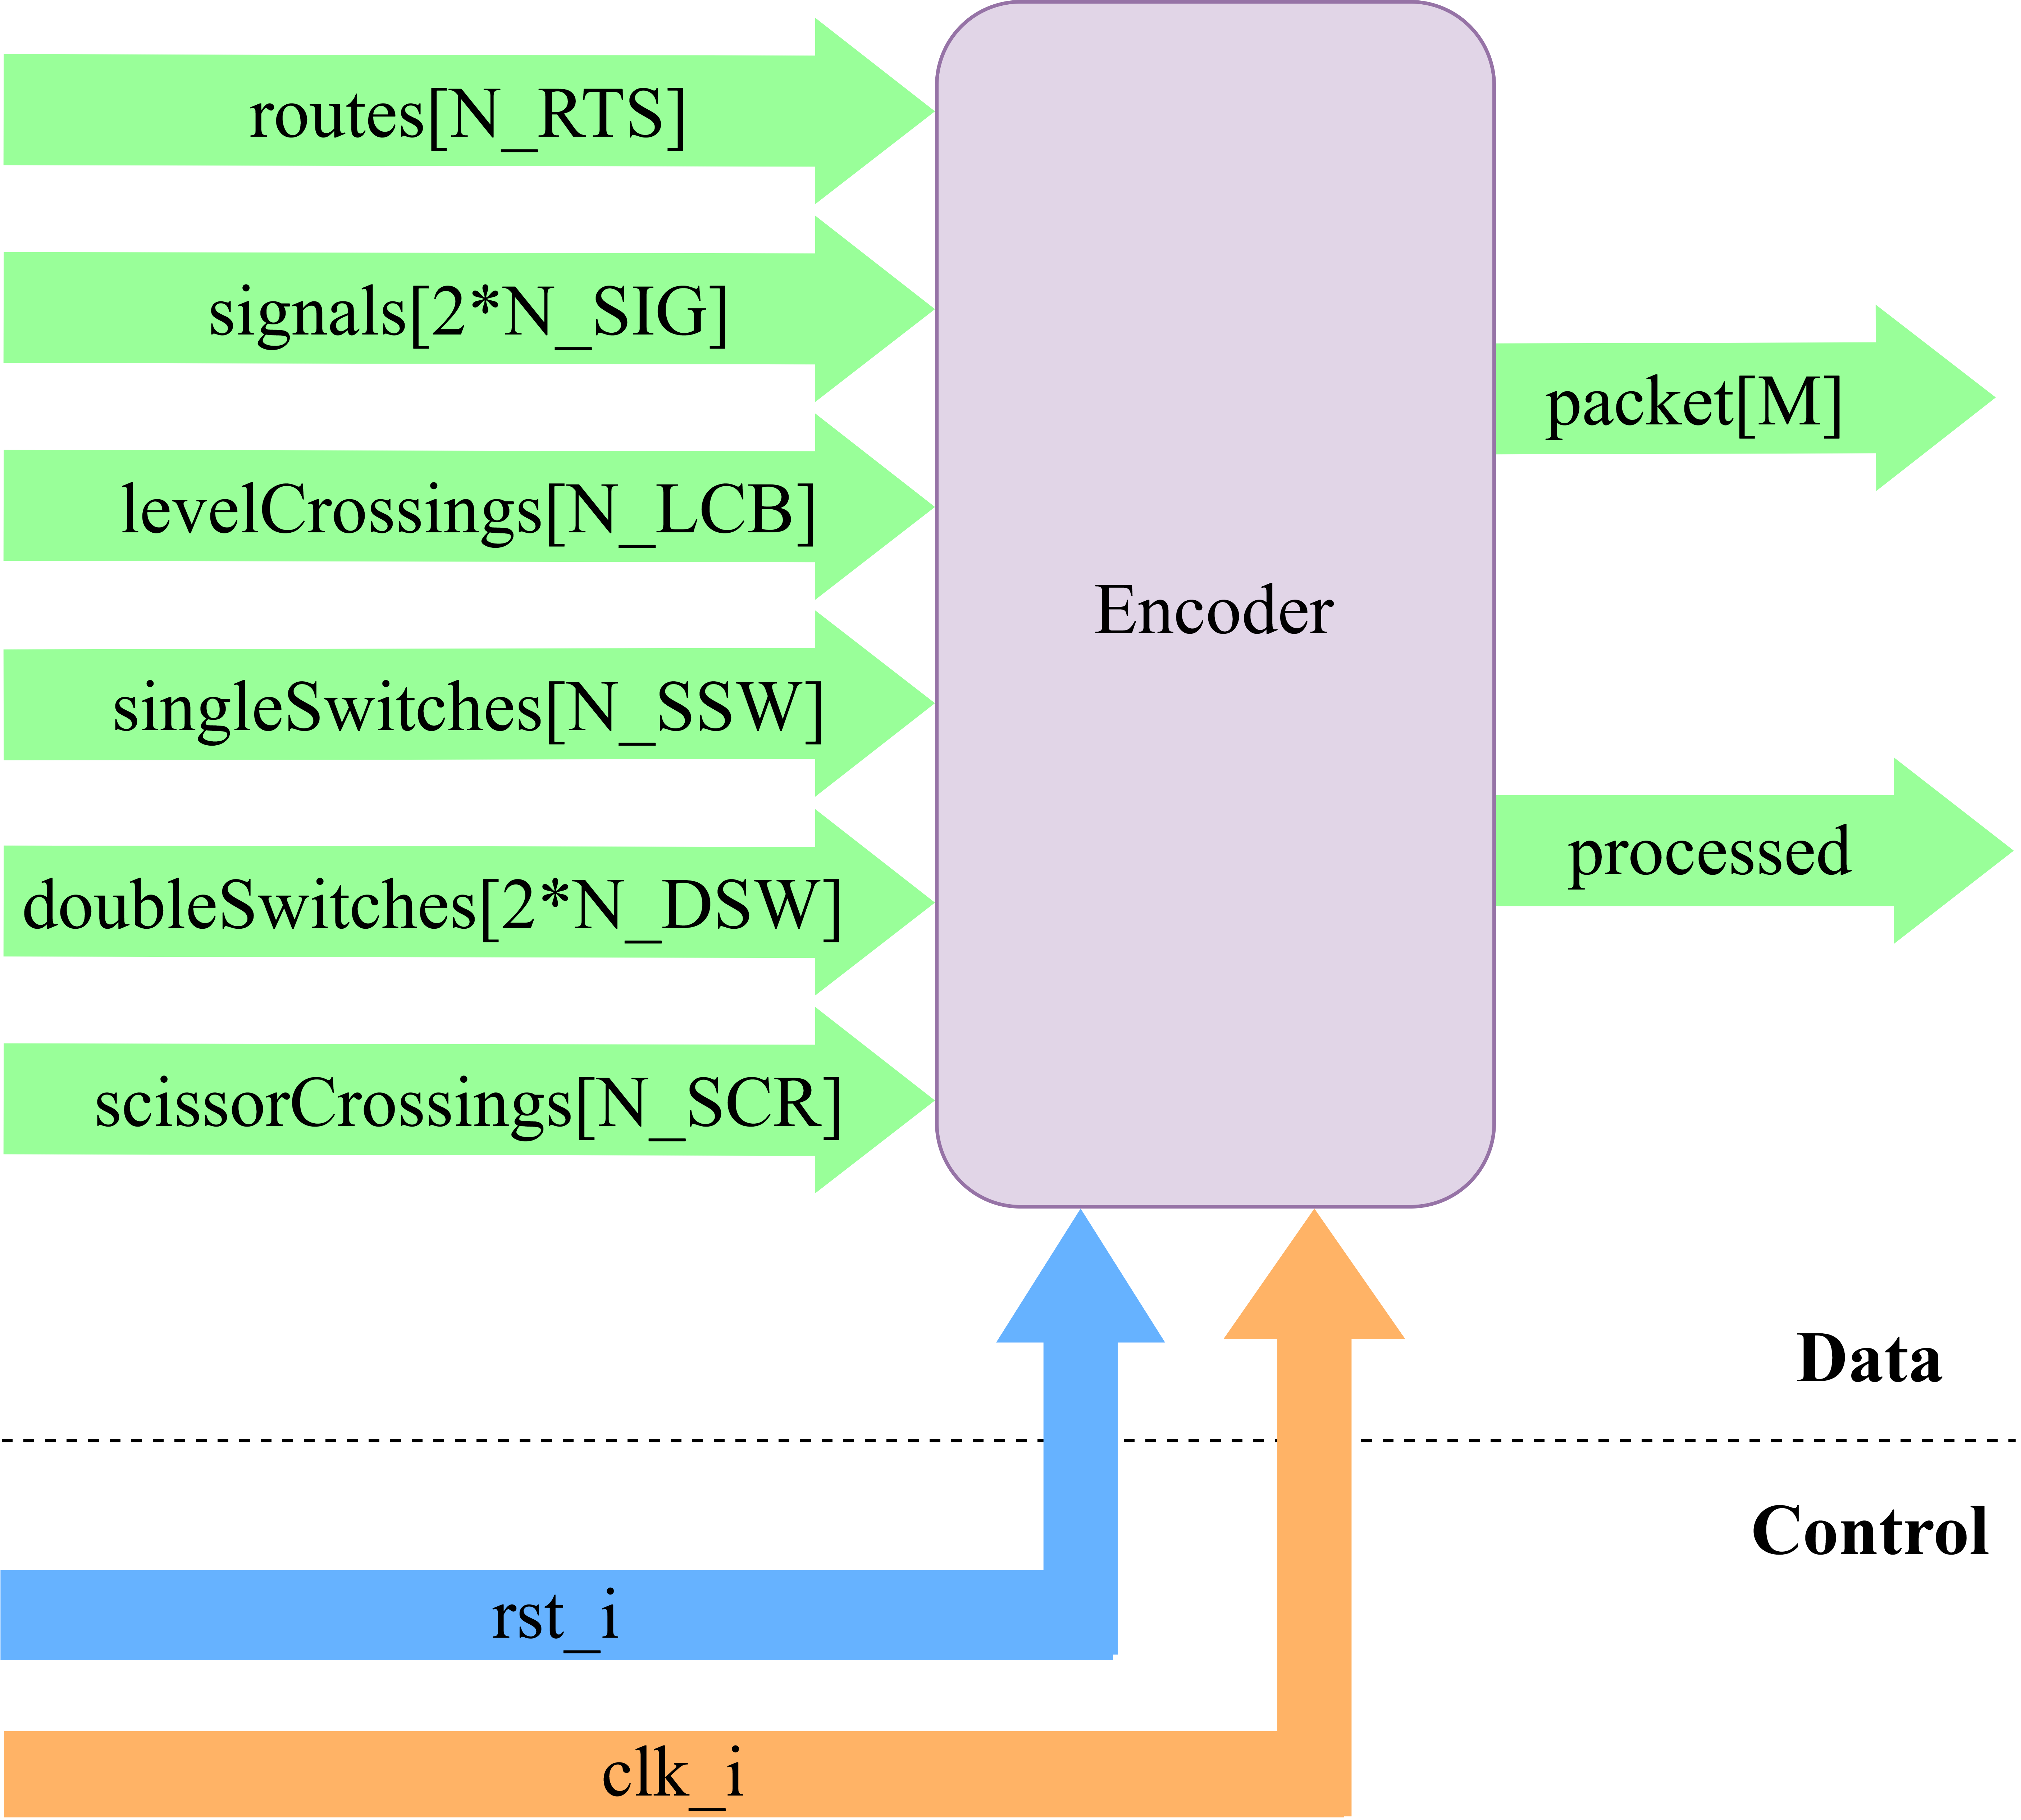
\includegraphics[width=1\textwidth]{Figuras/Encoder_module.png}
		\centering\caption{FSMD del módulo \textit{Encoder}.}
		\label{fig:Encoder_module}
	\end{figure}
	
	Al igual que la demultiplexación que realiza el módulo \textit{Decoder}, la multiplexación se basa en la cantidad de elementos ferroviarios de cada tipo, calculdos por el ACG al definir la trama tal cual fue explicado en la Sección \ref{sec:UART}. Los elementos inexistentes en la locación no serán tenidos en cuenta para formar la nueva trama, reduciendo el tamaño de la misma al mínimo.
\subsection{Módulo Printer}
	\label{sec:printer}
	
	El módulo Printer (ver Figura \ref{fig:GeneralSystem}) realiza la conversión de cada elemento de un vector de M elementos hexadecimales (\textit{packet}[M], M elementos de 4 bits) en caracteres hexadecimales (1 byte). Cada elemento del vector es analizado en cada ciclo de reloj (clk\_i) y demultiplexado, de manera tal de convertir un elemento por vez, para luego enviar el byte correspondiente al módulo UART para su posterior transmisión al exterior. El diagrama de bloques de la máquina de estados finitos con camino de datos se muestra en la Figura \ref{fig:Printer_module}.
	
	\begin{figure}[H]
		\centering
		\includegraphics[width=1\textwidth]{Figuras/Printer_module.png}
		\centering\caption{FSMD del módulo \textit{Printer}.}
		\label{fig:Printer_module}
	\end{figure}
	
	En cada ciclo de reloj el módulo \textit{Printer} demultiplexa el vector \textit{packet}[M] para obtener un elemento lógico que procesar, según el valor del contador vigente, que se incrementa en cada ciclo, hasta un máximo de M-1. Si el elemento \textit{packet}[i] es un valor hexadecimal, se enviará un byte equivalente en ASCII. Por ejemplo, se enviará un byte equivalente al 'A' ASCII si el elemento \textit{packet}[i] es una 'A' hexadecimal.
	
	Cada dos ciclos de reloj el módulo \textit{Printer} genera un pulso para habilitar el envío del último byte generado. Junto con el caracter se envía la señal \textit{wr\_uart} para indicarle a la UART que ese dato debe ser guardado en la FIFO de salida y la señal \textit{processed} para indicarle al módulo \textit{Detector} que se pueden procesar nuevas tramas. El ciclo de procesamiento de la trama a transmitir se describe el diagrama de estados de la Figura \ref{fig:Printer_FSMD}.
	
	\begin{figure}[H]
		\centering
		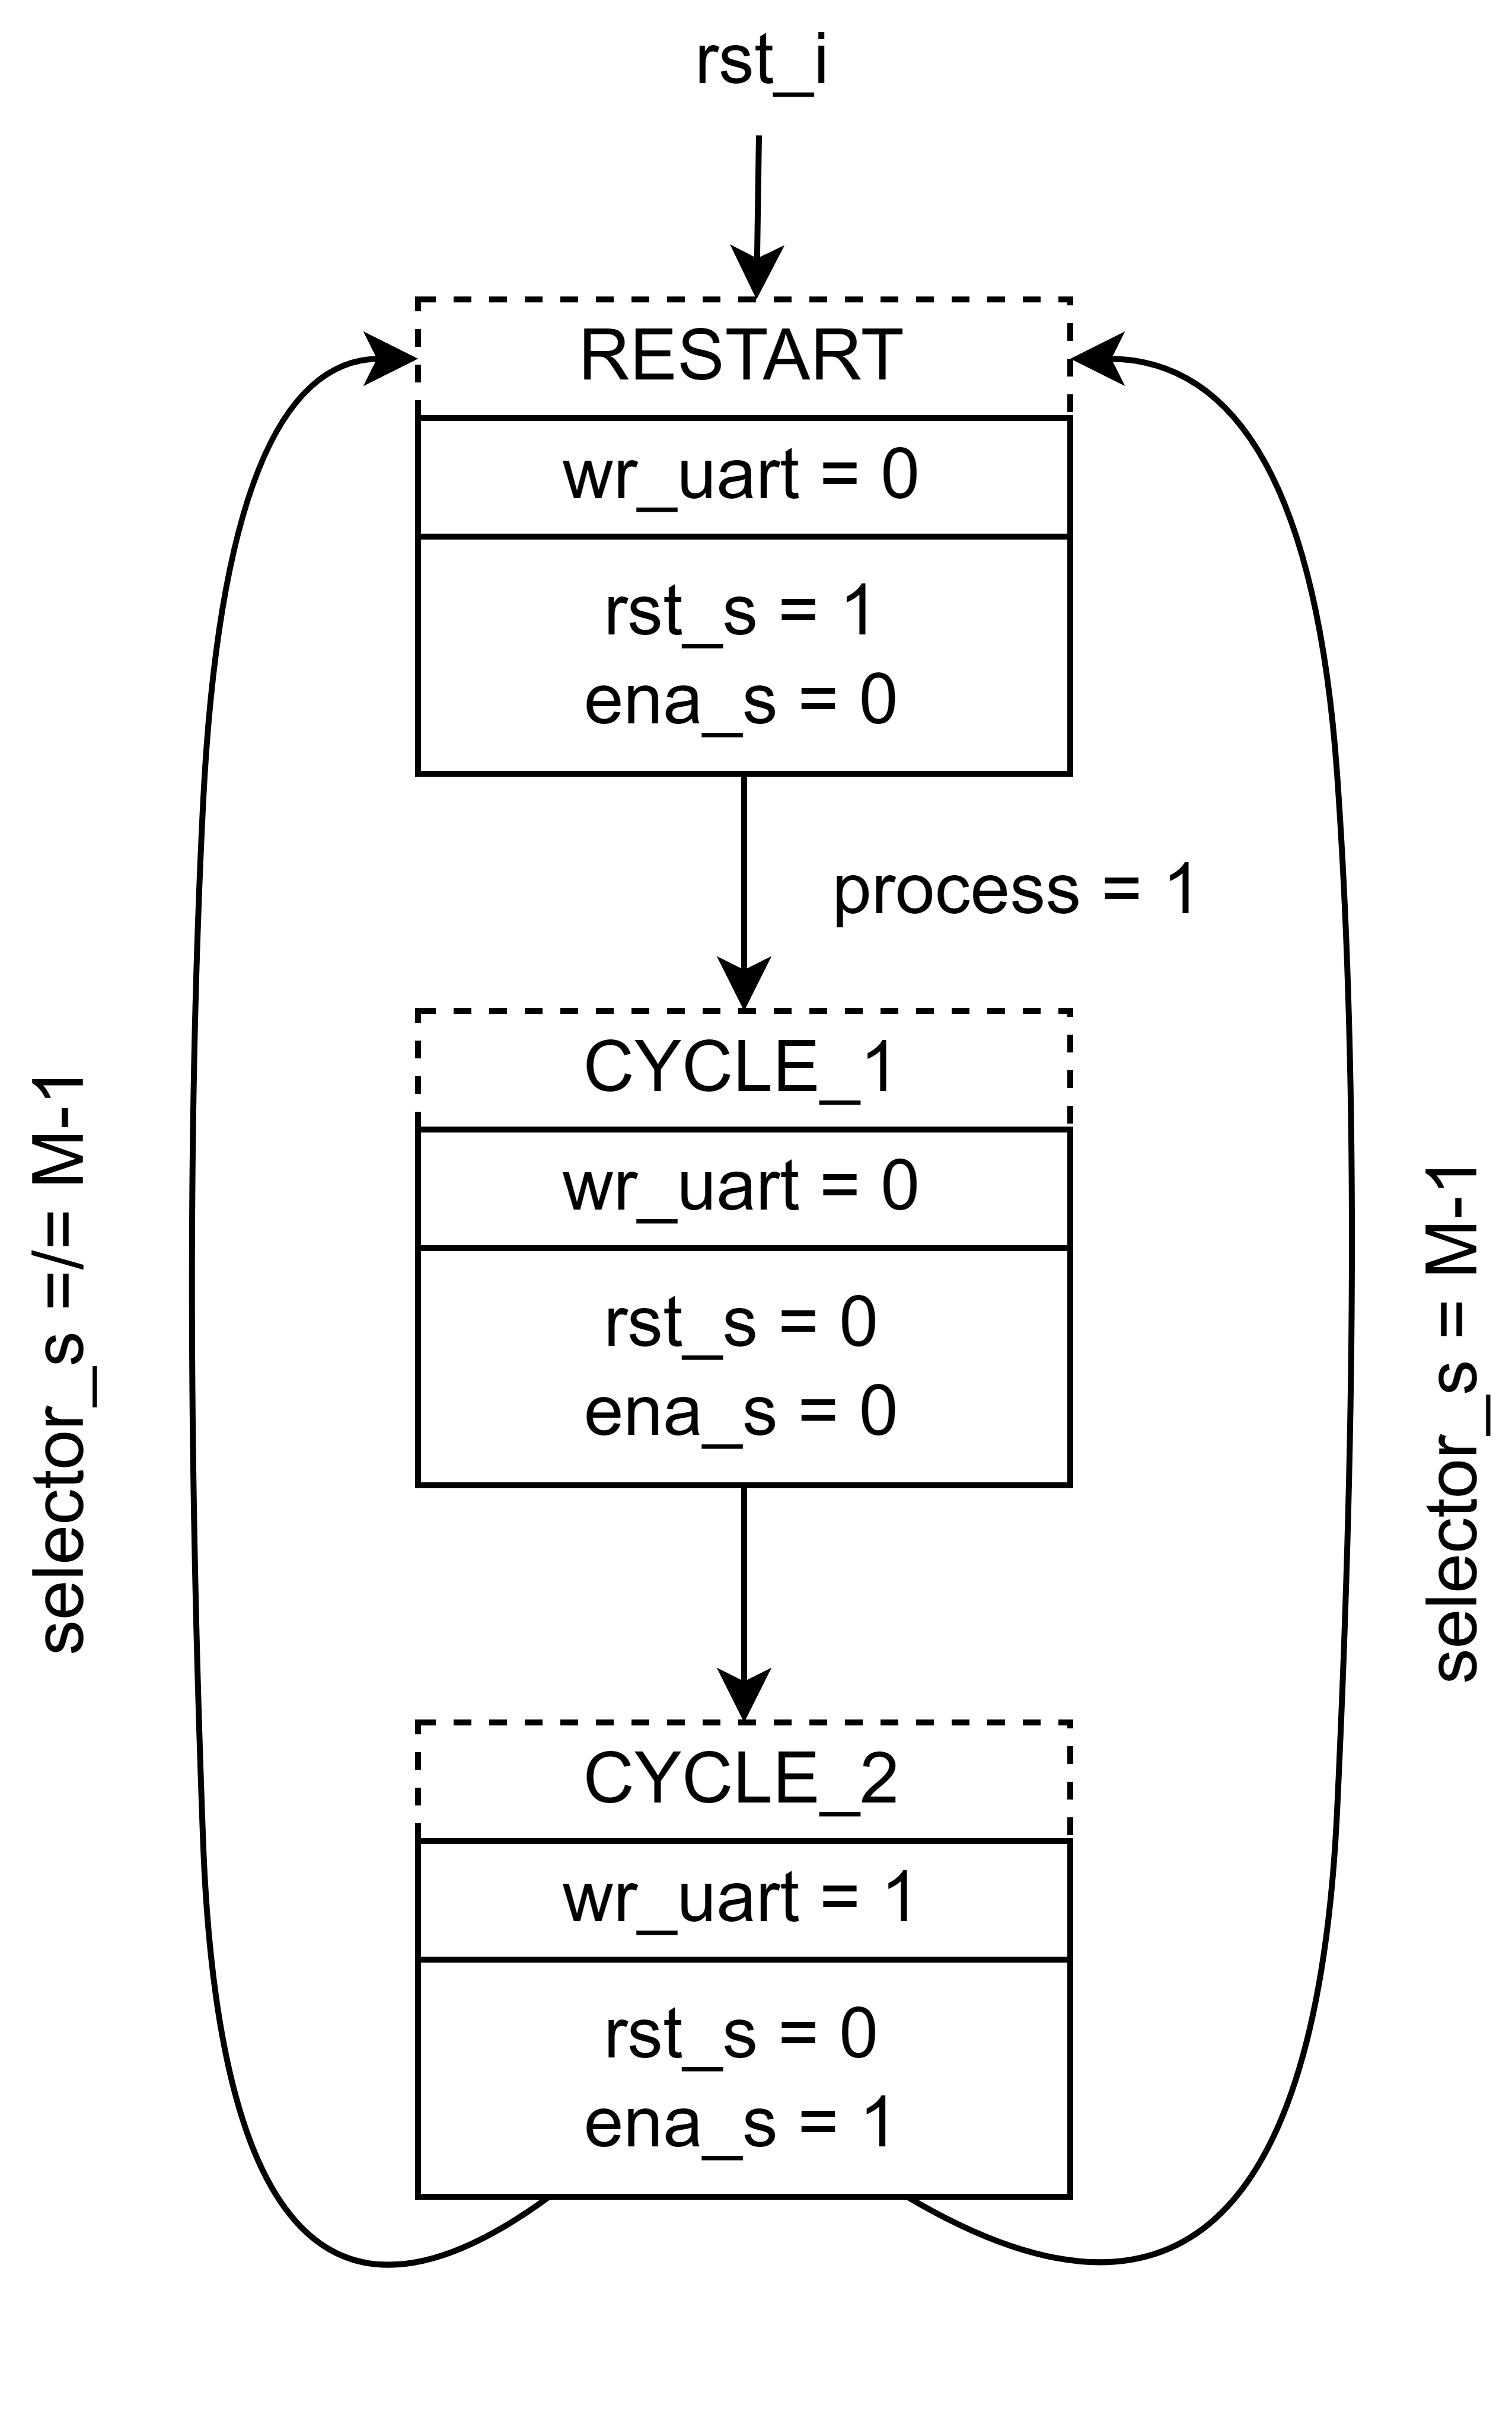
\includegraphics[width=0.8\textwidth]{Figuras/Printer_FSMD.png}
		\centering\caption{Diagrama de estados del módulo \textit{Printer}.}
		\label{fig:Printer_FSMD}
	\end{figure}
	
	El módulo \textit{Printer} inicia por detecto en el estado \textit{restart}, a la espera de recibir la señal \textit{process} del módulo \textit{Encoder}. Se tienen dos estados (\textit{cycle\_1} y \textit{cycle\_2}) para generar el pulso de reloj necesario para mantener sincronizadas las tramas. Cuando el contador haya recorrido los M elementos de \textit{packet}[M], el módulo vuelve al estado \textit{restart}, para esperar una nueva señal \textit{process} para volver a procesar una nueva trama de datos.
	
	Si la trama recibida es incorrecta, o si ya fue impresa, entonces la señal \textit{process} será '0' y el modulo \textit{Printer} dejará de enviar datos a la UART. Si la señal \textit{process} mantiene un estado lógico positivo, el proceso de impresión continuará hasta que la UART indique que no pueda recibir mas datos o que alguna etapa previa informe de algún error en el proceso.
\subsection{Módulo Selector}
	\label{sec:selector}
	
	Se añadió el módulo \textit{Selector} (ver Figura \ref{fig:GeneralSystem}) para poder facilitar el testeo de la comunicación serial al permitir anular la totalidad del sistema de enclavamiento. De esta manera, es posible validar la lectura, detección y escritura de tramas en bucle en forma independiente al sistema de enclavamiento. Esta funcionalidad es habilitada cambiando la posición de un switch físico de la FPGA y se desactiva invirtiendo su posición. El diagrama de bloques de la máquina de estados finitos con camino de datos diseñado para lograr este objectivo se muestra en la Figura \ref{fig:Selector_module}.
	
	\begin{figure}[H]
		\centering
		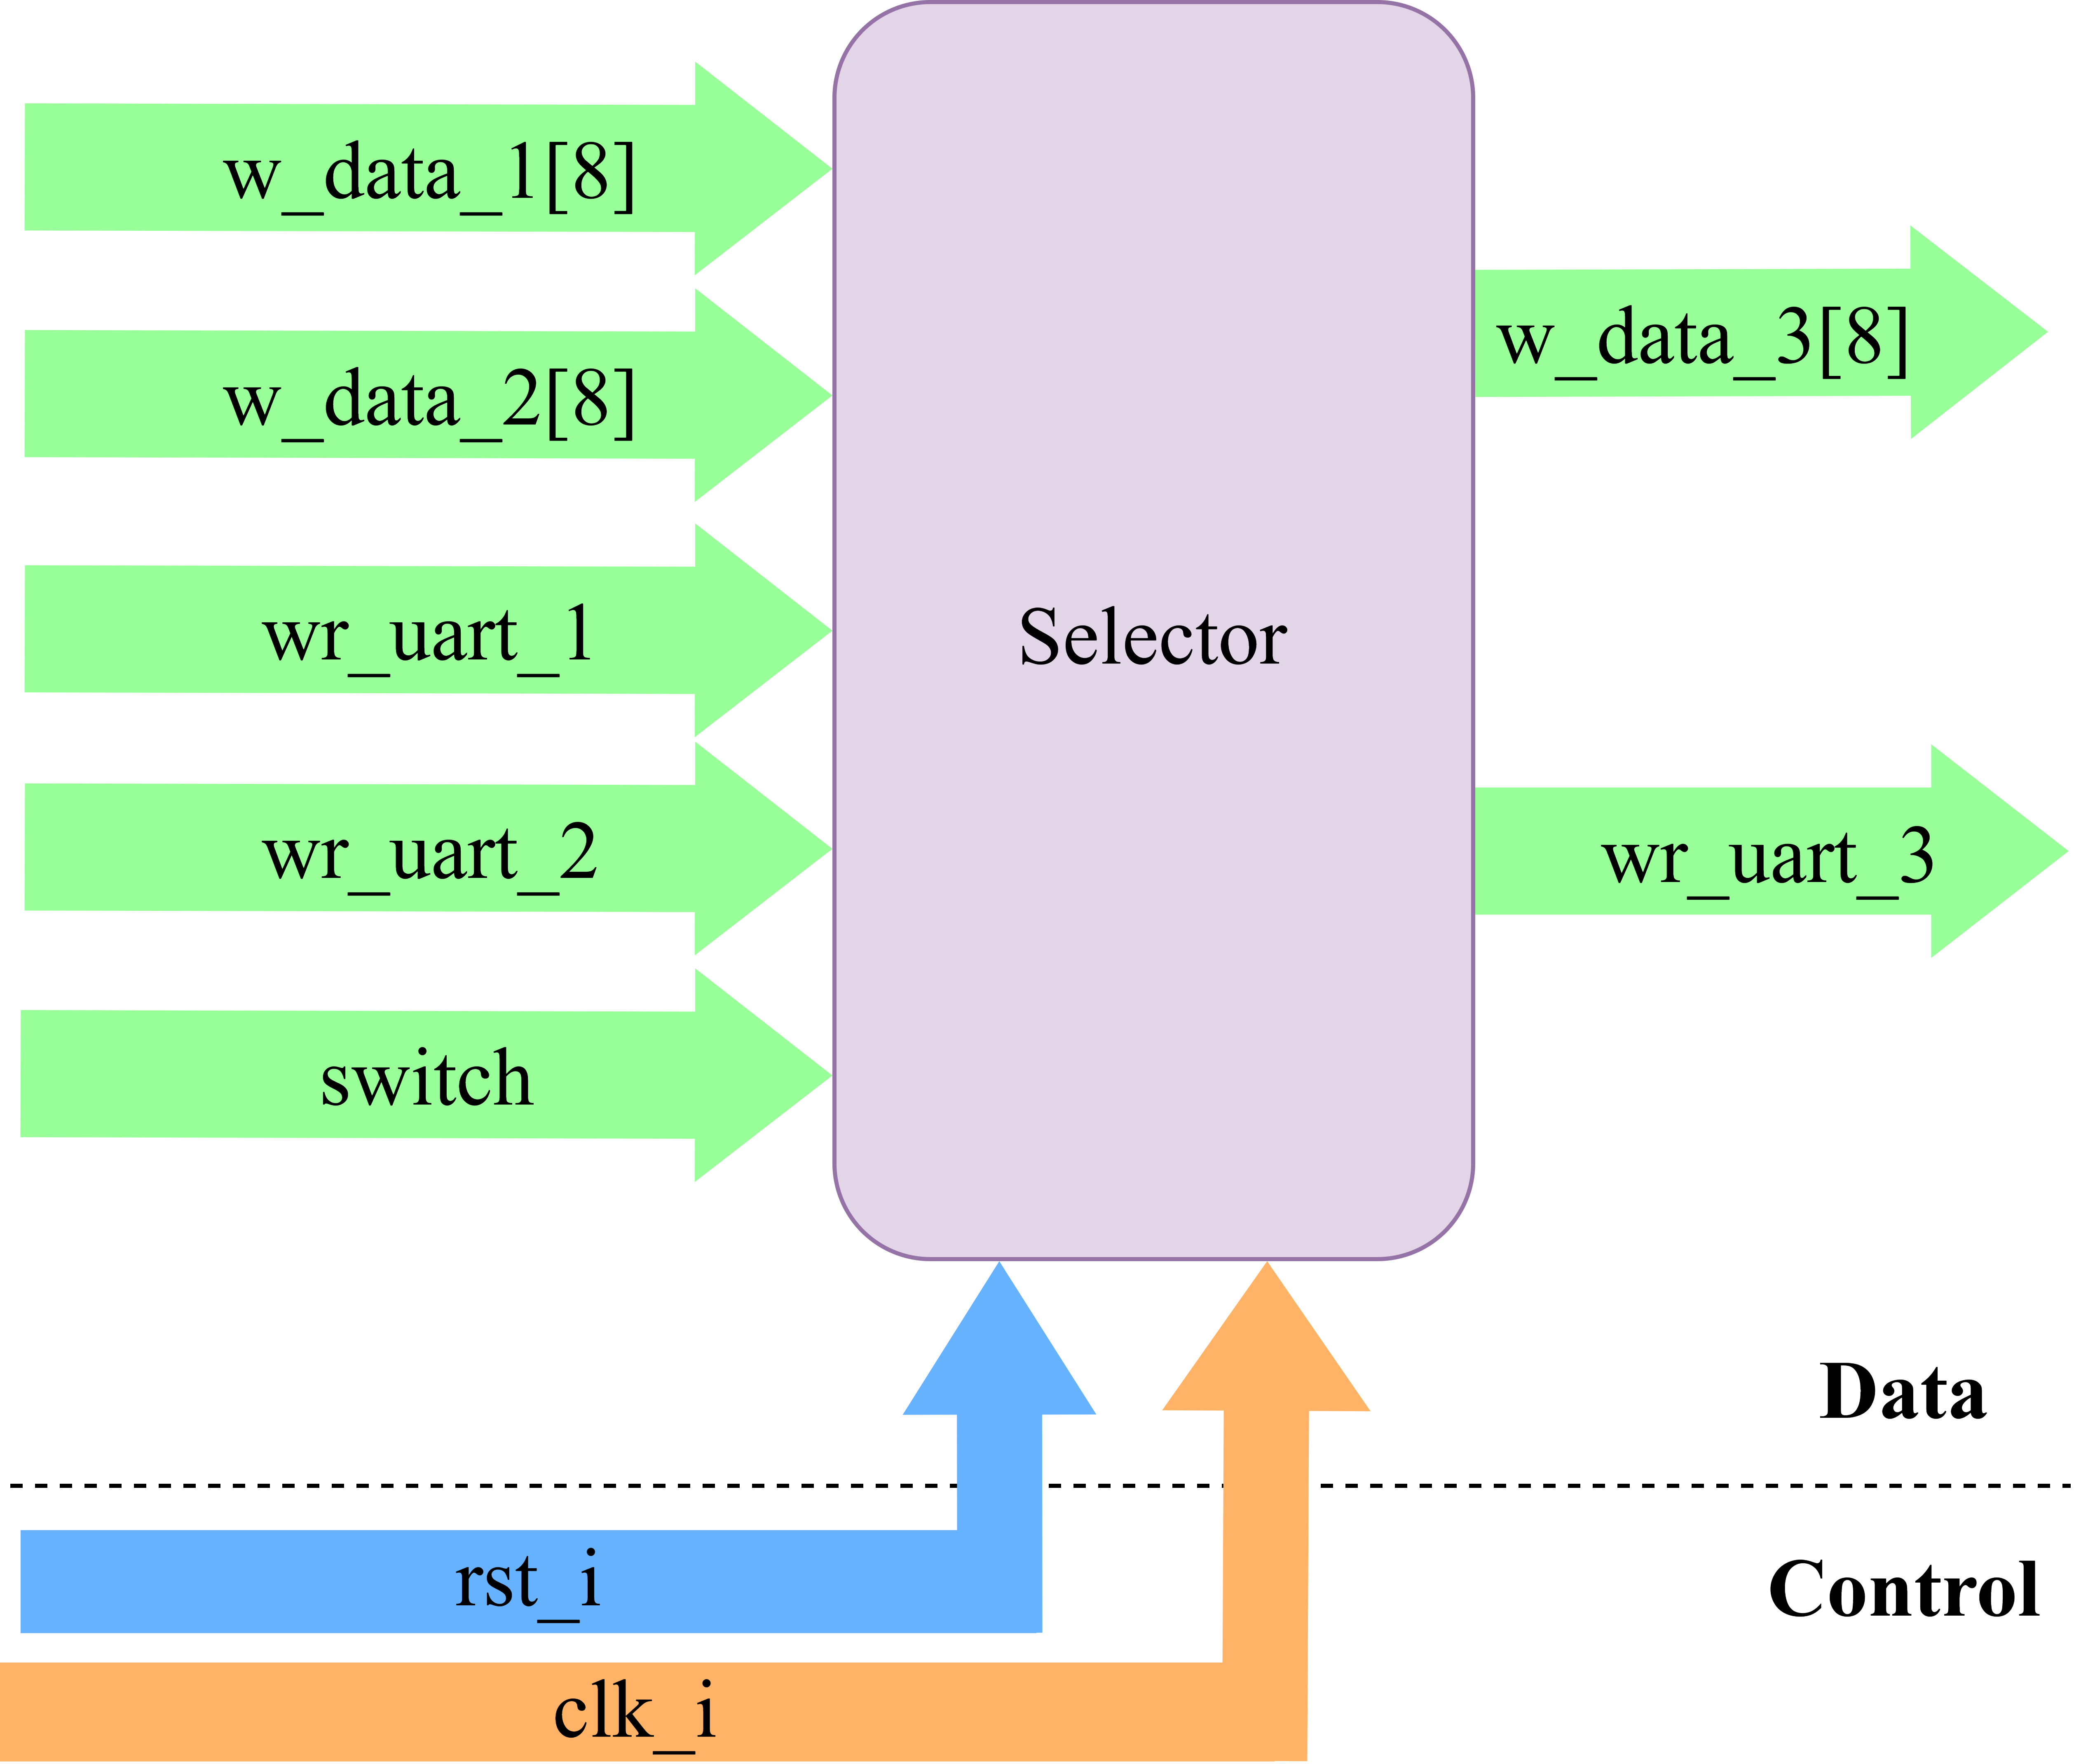
\includegraphics[width=0.55\textwidth]{Figuras/Selector_module.png}
		\centering\caption{FSMD del módulo \textit{Selector}.}
		\label{fig:Selector_module}
	\end{figure}